%--------------------------------------------------------------
% thesis.tex 
%--------------------------------------------------------------
% Corso di Laurea in Informatica 
% http://if.dsi.unifi.it/
% @Facolt\`a di Scienze Matematiche, Fisiche e Naturali
% @Universit\`a degli Studi di Firenze
%--------------------------------------------------------------
% - template for the main file of Informatica@Unifi Thesis 
% - based on Classic Thesis Style Copyright (C) 2008 
%   Andr\'e Miede http://www.miede.de   
%--------------------------------------------------------------
\documentclass[twoside,openright,titlepage,fleqn,
	headinclude,12pt,a4paper,BCOR5mm,footinclude]{scrbook}
%--------------------------------------------------------------
\newcommand{\myItalianTitle}{Intrusion Detection Systems and Machine Learning\xspace}
% use the right myDegree option
\newcommand{\myDegree}{Corso di Laurea Magistrale in Informatica\xspace}
%\newcommand{\myDegree}{
	%Corso di Laurea Specialistica in Scienze e Tecnologie 
	%dell'Informazione\xspace}
\newcommand{\myName}{Francesco Terrosi\xspace}
\newcommand{\myFaculty}{
	Scuola di Scienze Matematiche, Fisiche e Naturali\xspace}
\newcommand{\myUni}{\protect{
	Universit\`a degli Studi di Firenze}\xspace}
\newcommand{\myLocation}{Firenze\xspace}
\newcommand{\myTime}{Anno Accademico 2018-2019\xspace}
\newcommand{\myVersion}{Version 0.1\xspace}
%--------------------------------------------------------------
\usepackage[T1]{fontenc}
\usepackage{ellipsis}
\usepackage{pdfpages}
\usepackage{afterpage}
\usepackage{listings}
\usepackage{xcolor}
\usepackage{subfig}
\usepackage{caption}
\usepackage{appendix}
\usepackage{siunitx}
\usepackage[utf8]{inputenc}			%lettere accentate
\usepackage[italian]{babel}			%sillabazione italiana
\usepackage{amsmath}				%simboli matematici
\usepackage{amsfonts}				%font matematici
\usepackage{amssymb}				%altri simboli matematici
\usepackage{tikz}					%grafica
\usepackage{esint}					%simboli matematici
%--------------------------------------------------------------
\usepackage{dia-classicthesis-ldpkg}
%--------------------------------------------------------------
% Options for classicthesis.sty:
% tocaligned eulerchapternumbers drafting linedheaders 
% listsseparated subfig nochapters beramono eulermath parts 
% minionpro pdfspacing
\usepackage[eulerchapternumbers,linedheaders,subfig,beramono,eulermath,
parts]{classicthesis}
%--------------------------------------------------------------
\newlength{\abcd} % for ab..z string length calculation
% how all the floats will be aligned
\newcommand{\myfloatalign}{\centering} 
\setlength{\extrarowheight}{3pt} % increase table row height
\captionsetup{format=hang,font=small}
%--------------------------------------------------------------
% Layout setting
%--------------------------------------------------------------
\usepackage{geometry}
\geometry{
	a4paper,
	ignoremp,
	bindingoffset = 1cm, 
	textwidth     = 13.5cm,
	textheight    = 21.5cm,
	lmargin       = 3.5cm, % left margin
	tmargin       = 4cm    % top margin 
}

\lstset{
  	frame=tb,
	language=Java,
  	aboveskip=3mm,
  	belowskip=3mm,
  	showstringspaces=false,
  	columns=flexible,
  	basicstyle={\small\ttfamily},
  	numbers=none,
  	breaklines=true,
  	breakatwhitespace=true,
  	tabsize=3
}
%--------------------------------------------------------------
\begin{document}
\frenchspacing
\raggedbottom
\pagenumbering{roman}
\pagestyle{plain}
%--------------------------------------------------------------
% Frontmatter
%--------------------------------------------------------------
%--------------------------------------------------------------
% titlepage.tex (use thesis.tex as main file)
%--------------------------------------------------------------
\begin{titlepage}
	\begin{center}
   	\large
      \hfill
      \vfill
      \begingroup
         
\includegraphics[scale=0.15]{logo/LOGO}\\
%			\spacedallcaps{\myUni} \\ 
			\myFaculty \\
			\myDegree \\ 
			\vspace{0.5cm}
         \vspace{0.5cm}    
         Multivariate Analysis \& Statistical Learning
      \endgroup 
      \vfill 
      \begingroup
      	\spacedallcaps{\myItalianTitle} \\ $\ $\\
	\bigskip
      \endgroup
      \spacedlowsmallcaps{\myName}
      \vfill
      \spacedlowsmallcaps{6326113}
      \vfill
      \vfill
      \myTime
      \vfill                      
	\end{center}        
\end{titlepage}
\pagestyle{scrheadings}
%--------------------------------------------------------------
% Mainmatter
%--------------------------------------------------------------
\pagenumbering{arabic}
% use \cleardoublepage here to avoid problems with pdfbookmark
%\footnotesize

\section{Introduction}

	\begin{frame}{Table of content}
	
	\begin{itemize}
		\item Introduction
		\vspace{0.3cm}
		\item Intrusion Detection Systems
		\item Analyzer Implementation
		\begin{itemize}
			\item[1)] Data Preprocessing
			\item[2)] Feature Selection
			\item[3)] Analysis
		\end{itemize}			
	\end{itemize}
	
	\end{frame}

	\begin{frame}
		\begin{center}
			\begin{Huge}
				INTRODUCTION
			\end{Huge}
		\end{center}
	\end{frame}
	
	\begin{frame}
		\begin{itemize}
			\item Nowadays, we are seeing an increasing reliance on Artificial Intelligence
			\vspace{0.3cm}
			\item Combined with the increasing knowledge on statistical techniques, such as Multivariate Analysis and Statistical Learning (which are translated in Computer Science as "Machine Learning") these tools are even more powerful
			\vspace{0.3cm}
			\item Statistical Learning and Computer Security together to build a system capable of detecting users' and programs' malicious behaviours (e.g. an antivirus that detect malicious programs in a system)
		\end{itemize}
	\end{frame}
	
	\begin{frame}
		\begin{itemize}
			\item Our focus will be on the preprocessing and the analysis of data, in order to build such a system
			\vspace{0.3cm}
			\item We need to classify users' (and programs') behaviours and to classify them in order to detect suspicious activities
			\vspace{0.3cm}			
			\item To do so, the Kddcup99 was used. It is a well known dataset in this field, consisting of web activities observed through a couple of months by a military company
			\vspace{0.3cm}
			\item The dataset is \emph{really} huge. This was the cause of some computational limitation for the research but, as you will see, good results have been achieved anyway
			\vspace{0.3cm}
			\item The dataset also offer a set consisting of a non-contiguous 10\% of the original data, that was used for the training phase
		\end{itemize}
	\end{frame}		
	
	\begin{frame}
		\begin{center}
			\begin{Huge}
				INTRUSION DETECTION SYSTEMS
			\end{Huge}
		\end{center}
	\end{frame}
	
	\begin{frame}
		\begin{block}{Intrusion Detection System}
			An IDS is a hardware/software module capable of detecting \emph{intrusions} in a computer system by analyzing information from various areas within a computer or a network
		\end{block}
		\vspace{0.3cm}
		\begin{block}{Intrusion}
			An \emph{intrusion} is the \emph{unauthorized} act of bypassing the security measures of a system
		\end{block}
	\end{frame}
	
	\begin{frame}
		\begin{figure}
			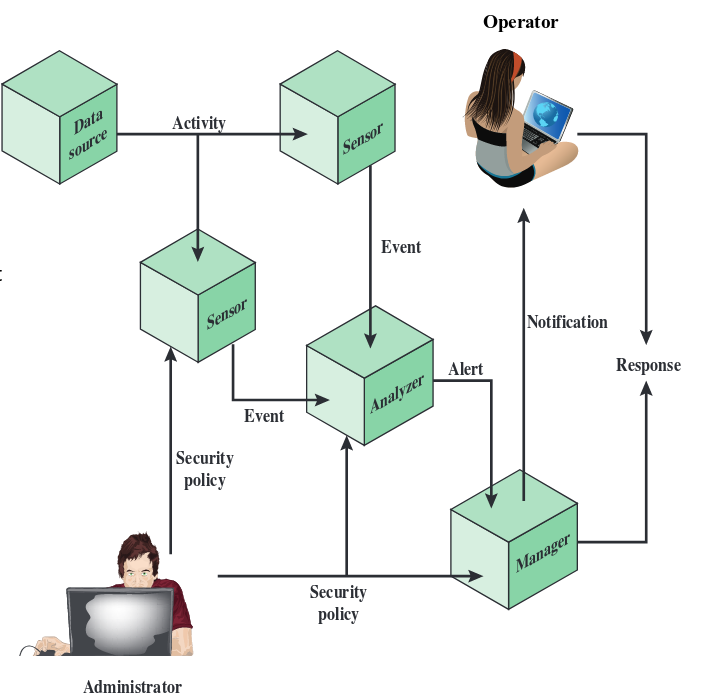
\includegraphics[width=\textwidth, height=0.85\textheight,keepaspectratio]{img/IDS.png}
		\end{figure}
	\end{frame}
	
	\begin{frame}
		Intrusion Detection System can be characterized on the basis of 2 aspects: the \emph{basing} of the system:
		\begin{itemize}
			\item Host-Based IDS
			\item Network-Based IDS
			\item Hybrid (Distributed) IDS
		\end{itemize}
		and on the techniques used for \emph{detection}:
		\begin{itemize}
			\item Signature-Based IDS
			\begin{itemize}
				\item[$\rightarrow$] We define a set of \emph{rules} that captures malicious behaviours
			\end{itemize}
			\item Anomaly-Based IDS
			\begin{itemize}
				\item[$\rightarrow$] We define the \emph{normal behaviours} and measure how close are the observed activities with respect to the model produced
			\end{itemize}
		\end{itemize}
		Can you see where Statistical Learning comes in? :)
	\end{frame}
	
	\begin{frame}
		Anomaly-Based IDS can use techniques based on Multivariate Analysis or Statistical Learning to develop the model of users' \emph{normal behaviour}\newline\newline
		Decision Trees are a good candidate for predictions since empirical results showed that this technique is one of the most accurate for intrusion detection\newline\newline
		Of course there are some drawbacks as:
		\begin{itemize}
			\item Data Gathering
			\begin{itemize}
				\item[$\rightarrow$] If you're not willing to use Stateful Protocol Analysis (i.e. you buy data from authorized vendors in order to build the model), you need sensors for data acquisition and you have to do some preprocessing
			\end{itemize}
			\item False-Positive/False-Negative rates
			\begin{itemize}
				\item[$\rightarrow$] Since intrusions are considered \emph{rare} (but often \emph{catastrophic}) events, we want to achieve the maximum accuracy possible
			\end{itemize}
		\end{itemize}
	\end{frame}
	
	\begin{frame}
		\begin{center}
			\begin{Huge}
				ANALYZER IMPLEMENTATION
			\end{Huge}
		\end{center}
	\end{frame}
	
	\begin{frame}
		\begin{itemize}
			\item An \emph{analyzer} for IDSs is a (typically) software module that collects data and raises an alarm if an intrusion is detected
			\item In this work, an hybrid Python/R software was developed:
			\begin{itemize}
				\item[1)] All the Preprocessing was done in Python for comodity (I'm quite familiar with it) and for the numbers of libraries available for Machine Learning
				\item[2)] The Decision Tree was built with R, using the rpart package
				\item[3)] Since R can work as a server to communicate with other process, there's no drawback on splitting modules using different languages (actually, this is often a requirement in software engineering!)
			\end{itemize}
			\item Data Analysis is a critical factor for achieving an high level of accuracy, thus multiple techniques were used for the process
		\end{itemize}
	\end{frame}
	
	\begin{frame}
	\vspace{0.5cm}
		Features' values in the dataset consist of heterogeneous types: we have integers, floats, strings\dots\newline\newline
		The first step is to convert all the values to a numeric type in order to proceed with the analysis! This is a very simple procedure an can be implemented straightforward by checking all the strings in the dataset
			\begin{figure}
				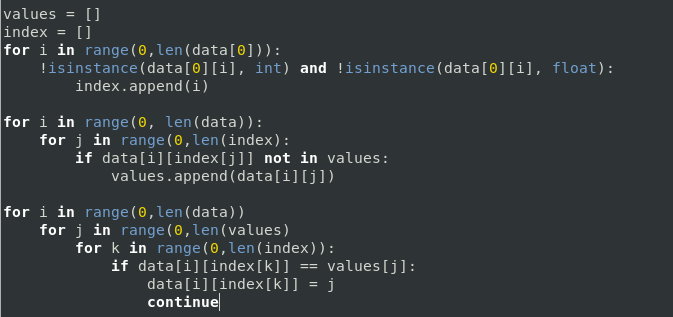
\includegraphics[width=\textwidth,height=0.85\textheight,keepaspectratio]{img/PreprocessCode.png}
			\end{figure}
	\end{frame}
	
	\begin{frame}
		The next step is features' standardization.\newline\newline This step is mandatory since Principal Component Analysis was used as a method for features' selection:
		\begin{center} If data are not standardized (i.e. scaled in order to associate to each feature a distribution with mean = 0 and variance = 1), there will be some features that appears to be the most relevant only because their values are of different scales\end{center}
		 (e.g. error rates, or rates in general usually shrink [0,1], while durations, number of requests etc are positive natural numbers)\newline\newline
		 \begin{itemize}
		 	\item[$\times$] The very important thing in this step is that we need to standardize both the test and the train set, which consists of different features' values, using the same criteria
		 	\item[$\bigstar$] Luckily for us, there is a Python library that implements all these operations for us: the Pandas library
		 \end{itemize}
	\end{frame}
	
	\begin{frame}
		\begin{figure}
			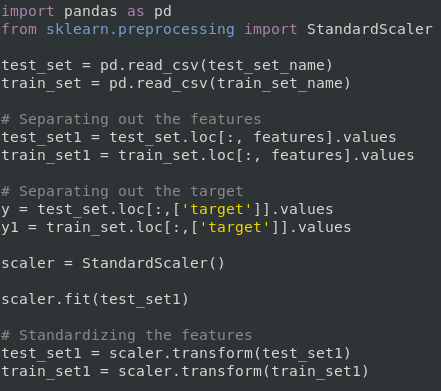
\includegraphics[width=\textwidth,height=0.8\textheight,keepaspectratio]{img/Normalization.png}
		\end{figure}
	\end{frame}
	
	\begin{frame}
		After data have been standardized, we need to select only the relevant features in the dataset (since it consists of 40 variables!)\newline\newline
		To do so, a Principal Component Analysis was conducted on the dataset.
		\begin{block}{PCA}
			\begin{itemize}
			
				\item It is a technique that uses algebra calculations to reduce the number of variables in a dataset
				\item First of all, the variance-covariance matrix $V$ must be computed
				\item Then, we need to calculate its eigenvectors and eigenvalues, that translates into solving the equation: $det( V - \lambda I) = 0$
				\item These vectors represent "new" features that explain the variance of the variables in the dataset
				\item You then choose the number of components (the vectors) you need to preserve the accuracy of the representation of the original dataset
			\end{itemize}
		\end{block}
	\end{frame}
	
	\begin{frame}
		Here we have the same problem we had with standardization: if we perform some transformation on the train-set, the \emph{same} transformation must be done on the test-set and on the real data you will gather from sensors.\newline\newline
		Luckily, again, the Pandas library comes in help:
		\begin{figure}
			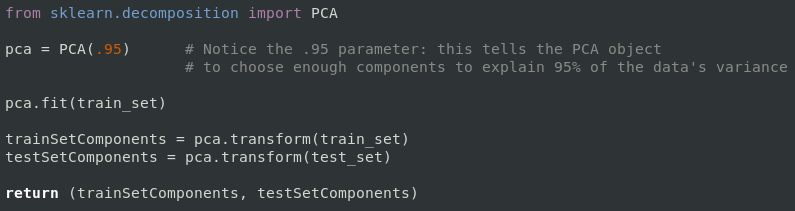
\includegraphics[width=\textwidth,height=\textheight,keepaspectratio]{img/PCA.png}
		\end{figure}
	\end{frame}
	
	\begin{frame}
		Now that data are cleaned, standardized and the principal components were calculated, we can start building the Decision Tree!\newline\newline
		Decision Trees are statistical models that can be used for classification and the analysis of variance.\newline\newline
		In this research we are most interested in classification since we want to classify \emph{bad} and \emph{good} users. In the next block is briefly described the algorithm to build a DT
		\begin{block}{Decision Tree Construction}
			\begin{itemize}
				\item For each variable we split the dataset in 2 groups (e.g. using the Gini Index metric)
				\begin{itemize}
					\item[$\rightarrow$] Since our variables are continuous, splits will be done on boolean conditions, that is: given a threshold \emph{t}, we will check the features whose value is greater than \emph{t} and the ones lower than \emph{t}
				\end{itemize}
				\item The variable (feature) that produced the "best" score will be the very first split (i.e. the root of the tree)
				\item The algorithm now proceeds recursively on each node, until a certain alt condition is met (e.g. all the variables have been chosen for splitting the dataset)
			\end{itemize}
		\end{block}
	\end{frame}
	
	\begin{frame}
		The DT was built using R, since it is faster than Python and, if our train-set is about 200 MB, our test-set is 2 GB, so considerations on performances led me thowards R\newline\newline
		Decision Trees can be built using the package \emph{rpart}. It offers many parameters to tell the algoirthm how to build it such as the variables that need to be considered and the complexity parameter (i.e. the tree \emph{depth})\newline\newline
		It also provides a function for predictions over a dataset. The output of this predictions are used to compute the \emph{Confusion Matrix}
		
\begin{center}
	{\setlength{\extrarowheight}{20pt}
	\begin{tabular}{| c | c  c |}
	\hline
		 & Actual values & \\ \hline
		Predictions & True & False  \\ \hline
		True & True Positive & False Positive \\ \hline
		False & False Negative & True Negative \\ 
		\hline
	\end{tabular}}\par
	\bigskip
	
	\begin{tiny}
		Simple $2x2$ confusion matrix example
	\end{tiny}
	\end{center}
	\end{frame}
	
	\begin{frame}
		The confusion matrix can be used to calculate the accuracy of predictions over a dataset. The formula is quite straightforward and is shown, together with the tree construction, in the figure below:
		
		\begin{figure}
			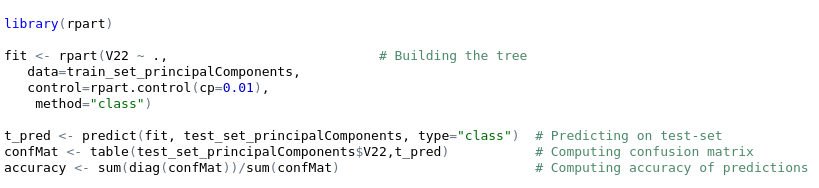
\includegraphics[width=\textwidth,height=\textheight,keepaspectratio]{img/Rpart.png}
		\end{figure}
	\end{frame}
	
	\begin{frame}
		\begin{center}
			\begin{Huge}
				RESULTS \& CONCLUSIONS
			\end{Huge}
		\end{center}
	\end{frame}
	
	\begin{frame}
		The Decision Tree was built using different three different representation of the same train-set.\newline\newline
		The Kddcup99 dataset provides a file which consists of a 10\% of the original dataset (the rows in this smaller dataset are not contiguous in the original dataset)\newline\newline
		For technical reasons, this small file was used as a train-set (usually train-sets are about the 70/80\% of the original file)\newline\newline
		For complexity parameters equal to 0.01, 0.0025 and 0.001, the algorithm was given as input:\newline
		\begin{itemize}
			\item[1)] The preprocessed dataset (i.e. strings are replaced and values are standardized, all the features in input)
			\item[2)] The features \emph{selected} by PCA (this is, indeed, a non-standard use of PCA)
			\item[3)] The new features \emph{produced} by PCA
		\end{itemize}
	\end{frame}
	
	\begin{frame}
		\begin{center}
	{\setlength{\extrarowheight}{20pt}
	\begin{tabular}{| c | c | c | c |}
	\hline
		Complexity parameter & 0.01 & 0.0025 & 0.001 \\ \hline
		StandardizedKddcup & 0.9870385 & 0.9832191 & 0.9843356 \\ \hline
		KddcupPrincipalFeatures & 0.9849946 & 0.9948412 & 0.9963878 \\ \hline
		PCA eigenvectors & 0.9901552 & 0.9951242 & 0.9956888 \\ 
		\hline
	\end{tabular}}
\end{center}
	\end{frame}
	
	\begin{frame}
		\begin{block}{Standardized Kddcup}
			\begin{itemize}
				\vspace{0.3cm}
				\item The Decision Tree ran over the whole set of features, is the one with the lowest accuracy
				\vspace{0.3cm}
				\item This Tree is also very susceptible to the complexity parameter: bigger trees mean lower accuracy (as you could see from the previous table)
				\vspace{0.3cm}
				\item Trees built with this dataset are also very much unbalanced with respect to the others
				\vspace{0.3cm}
			\end{itemize}
		\end{block}
	\end{frame}
	
		\begin{frame}
		\begin{block}{Restricted Feature Set Standardized Kddcup}
			\begin{itemize}
				\vspace{0.3cm}
				\item This train-set consist of the features chosen by the PCA, but the values used are the ones of the \emph{original} dataset
				\vspace{0.3cm}
				\item Despite the fact that this is not the standard usage of PCA, these trees show pretty good accuracy (actually, greater complexity lead to higher accuracy with respect to PCA trees)
				\vspace{0.3cm}
				\item However, this could be a consequence of using only the 10\% of the original dataset as a train-set
				\vspace{0.3cm}
				\item Regarding the Tree Structure, these ones are very similar to the PCA trees
				\vspace{0.3cm}
			\end{itemize}
		\end{block}
	\end{frame}
	
	\begin{frame}
		\begin{block}{PCA features}
			\begin{itemize}
				\vspace{0.3cm}
				\item The last train-set is the output of the PCA algorithm
				\vspace{0.3cm}
				\item The drawback of this approach is that, since we changed the original features' set, we have to transform the test-set, as well as any other value that will be used for future predictions (remember we had to \emph{fit} the PCA object in Pandas?)
				\vspace{0.3cm}
				\item The accuracy of these trees is similar to the previous one, but the gain in accuracy is lower when we increase the complexity (i.e. decrease the complexity parameter)
				\vspace{0.3cm}
				\item Just like the previous trees, these ones are very well balanced and do not suffer bigger structures
				\vspace{0.3cm}
			\end{itemize}
		\end{block}
	\end{frame}
	
	\begin{frame}
		***TREE PLOTS***
	\end{frame}
	
	\begin{frame}
		\begin{center}
			\begin{Huge}
				THANKS FOR YOUR ATTENTION
			\end{Huge}
		\end{center}
	\end{frame} % use \myChapter command instead of \chapter
\tableofcontents
\clearpage
\chapter{Introduction}
	
Nowadays, we are seeing how much reliance is put into Artificial Intelligence, especially when statistical techniques come in.\newline
The combination of AI and MASL (known as Machine Learning in computer science), gives us a set of very powerful tools in order to accomplish the hardest objectives. Most of the times, these techniques are used for financial business but what happens when we try to apply Machine Learning to Computer Security?\newline
In this paper we will see how powerful can be statistical models when applied to computer security, how they can be applied and in what field and what are the techniques to be used and the steps to build a resilient and secure system.\newline
The focus will be on Intrusion Detection and Prevention System (roughly, you can think to an Anti-Virus as an IPS) based on Anomaly Detection techniques.\newline
Anomaly Detection relies on defining a model for the \emph{normal} behaviour of a user into a system and comparing the observed behaviour of actual users (or programs) with the established model, in order to detect attacks and intrusion. for sake of understanding, you can think to a malware (e.g. a virus) as a "bad user" trying to gain control of your computer system.\newline\newline

In this paper we will go through these topics:
\begin{itemize}
	\item A general overview of Intrusion Detection and Prevention Systems
	\item An overview of the techniques used for \emph{Feature Selection}
	\item An overview of the techniques used for \emph{Classification}
	\item A practical implementation
\end{itemize}


\chapter{Intrusion Detection and Prevention Systems}

Intrusion Detection (and Prevention) Systems (from now on, IDS and/or IPS) are particular HW/SW systems developed to detect security threats in a computer system.\newline
Historically, they were developed using signature-based techniques, that is: you define an attack pattern and, if ot recognize that exact pattern in the system's activity, it raises an alarm.\newline\newline
Since Machine Learning is one of the increasing trends, gaining more and more popularity, we began to think if, instead of defining the "attack pattern" (or signature) for a particular malicious activity, we could define the "good behaviour" for users and program to detect malicious behaviour and here is where anomaly-based IDS comes in.

\subsection{Machine Learning and IDS combined}

Let's get more into the interesting things now. The first question is: How do I define the "normal" behaviour for users and programs? We need to have a dataset representing these behaviours. We have two alternatives:

\begin{itemize}
	\item Stateful Protocol Analysis
		\begin{itemize}
			\item[$\rightarrow$] We buy these datasets from authorized vendors. These data are usually very accurate and very little work is needed on them. The bad thing? The price is usually very high
		\end{itemize}
	\item Collect data by ourselves
		\begin{itemize}
			\item[$\rightarrow$] This approach is usually less expensive but require much more work on the data (such as \emph{feature selection}). For the purpose of this course we will have a better look at this approach, since it allows us to use some more statistical techniques
		\end{itemize}
\end{itemize}

Data are collected by the IDS using a \emph{sensor} (an HW or SW module). These data are sent to an \emph{analyzer} that compares them with the ones collected in the training phase, in order to detect intrusions. However, the very big problem with these kind of systems is that we want a very small number of \emph{false positives} and \emph{false negatives}, otherwise the whole system is useless!\newline\newline
This is the main reason why we will put some emphasis to \emph{feature selection} and \emph{feature classification}\newline\newline

Roughly, the process used to build this kind of system is depicted in Figure 1:
	\begin{itemize}
		\item[1)] First of all we need a \emph{Train Set}, to tell the system what are the accepted behaviours
		\item[2)] Now that we have only the relevant components in our train set, we can classify data. Empirically, it has been observed that \emph{Decision Tree} provides the higher accuracy for anomaly detection
		\item[3)] At this point we are able to test our system with a \emph{Test Set}, to check the accuracy of our model of correctly detecting intrusions
	\end{itemize}
	
	\begin{figure}[h!]
		\centering
		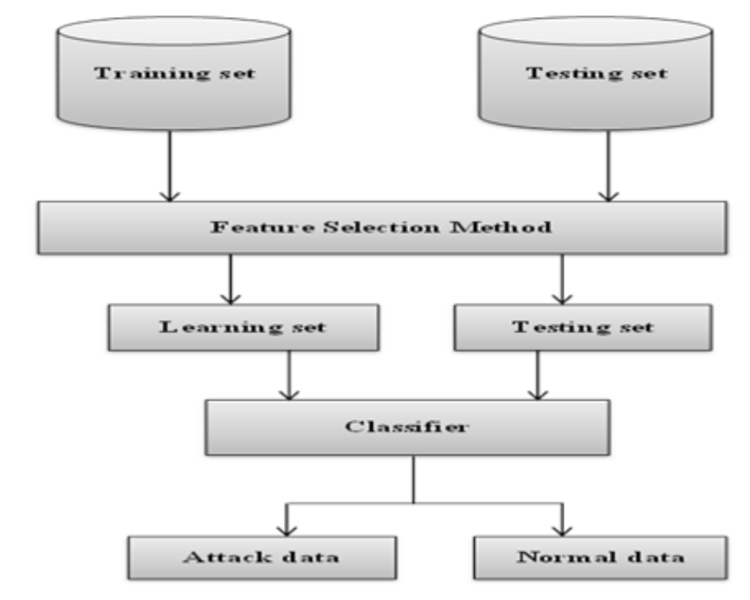
\includegraphics[width=\textwidth,height=8.5cm]{img/IDSPhases.png}
	\end{figure}
\chapter{Feature Selection}

Feature selection is, no doubt, the critical part when we need to prepare the dataset for the training phase.\newline
If one collects data for the training on its own (i.e. you don't buy data from authorized vendors), tipically they will have a lot of redundant attributes, a lot of useless attributes (for intrusion detection) and what he/she wants is to extract from all the observed data the most representative attributes for attacks and behaviours.\newline
In this section we will briefly describe the techniques that can be used and the pros and cons of each approach.

\begin{itemize}
	\item \emph{Principal Component Analysis} One of the most used techniques for determining uncorrelated attributes and the one that has been used in this implementation
	\vspace{0.3cm}
	\item \emph{Correlation Based Feature Selection Method} works under the hypothesis that: "Good feature subsets contain features higlhly correlated with the class, yet uncorrelated with each other"
	\vspace{0.3cm}
	\item \emph{Information Gain Based Feature Selection}: roughly, we combine entropy calculation and Information Gain to select the attributes that give us the more information about the class we want to predict
	\vspace{0.3cm}
	\item \emph{Minimum Redundancy Maximum Relevance} is an approach based on the assumption that the most redundant features are the less relevant ones.
\end{itemize}

\section{Principal Component Analysis}

Principal Component Analysis is a technique used for feature selection, which involves algebra techniques. The idea is to calculate the variance-covariance matrix and to calculate its eigenvectors and eigenvalues, in order to select the biggest ones (i.e. the ones that explain most of the variance in the dataset).\newline\newline
	
$
V = 
	\begin{pmatrix}
		\sigma_{1} & \sigma_{12} & \sigma_{13} & \dots & \sigma_{1n}\\
		\sigma_{21} & \sigma_{2} & \sigma_{23} & \dots & \sigma_{2n}\\
		\vdots & \vdots & \vdots & \vdots & \vdots\\
		\sigma_{n1} & \sigma_{n2} & \sigma_{n3} & \dots & \sigma_{n}\\
	\end{pmatrix}
$

Given this matrix, calculate $det(V\ -\ \lambda I)\ = \ 0$ to obtain all the eigenvectors and eigenvalues, and choose the "best" ones that is:\newline\newline
\begin{center}
 $max\ | x |_{x\ eigenvalue\ \in V}$\newline\newline
\end{center}
To use this techniques, it is \emph{very} important to scale data: through standardization (mean=0, variance=1) or normalization (make values shrink [0,1]). This is because PCA produces a number n of eigenvalues and eigenvector, representing for each feature the impact it has on variance. If we have values with very different scales, we could give much more importance to integer values than to, for example, a rate values.
\chapter{Classification Approaches}

A classifier is a tool that tries to categorize unseen patterns in suitable classes.\newline
An accurate (or a "good") train-set is crucial to build a model that provides the best accuracy to Anomaly Detection.\newline
The classifier uses the train-set to build the model that will be used to classify users (and programs) behaviour and to take decision about whether the observed actions are legitimate or not. Empirical studies will help in choosing the most accurate model (in terms of false-positives and false-negatives ratio)\newline\newline

Here there are the most used approached towards classification in Anomaly Detection:

\begin{itemize}
	\item \emph{Decision Trees} are certainly one of the most used and accurate tools for classification. It builds a model from a train-set that takes decision based on the comparison between the observed features and the nodes of the tree, starting from the root until reaching a decision (leaf) node
	\vspace{0.3cm}
	\item \emph{Nave Bayes} simply uses a form of Bayesian Network to infer intrusions
	\vspace{0.3cm}
	\item \emph{Support Vector Machine} is a technique in which we try to minimize the risk (but we sacrifice some accuracy) in order to optimize speed and scalability
	\vspace{0.3cm}
	\item \emph{Neural Network} is a "connectionist" approach that tries to simulate the human's brain with artificial (digital) neurons. The pros of this approach is, no doubt, its accuracy when the network is trained for a long period, consisting in multiple generations of NN. The cons is that if an error is made in the first generations, it will be propagated to the next ones
	\vspace{0.3cm}
	\item \emph{K-Nearest Neighbours} is the simplest approach (but surprisingly one of the most accurate in the field of Intrusion Detection!) among all these Machine Learning techniques. The idea is to classify "patterns" instead of features
\end{itemize}

Collecting some results from empirical studies, here it is a comparison table from all these classification approaches combined with the feature selections technique. As can be seen, the \emph{Decision Tree} classification technique is the one with the \emph{overall} best accuracy.\newline
On the other hand we got the best accuracy combining K-NN with Information Gain

\begin{figure}[h!]
	\centering
	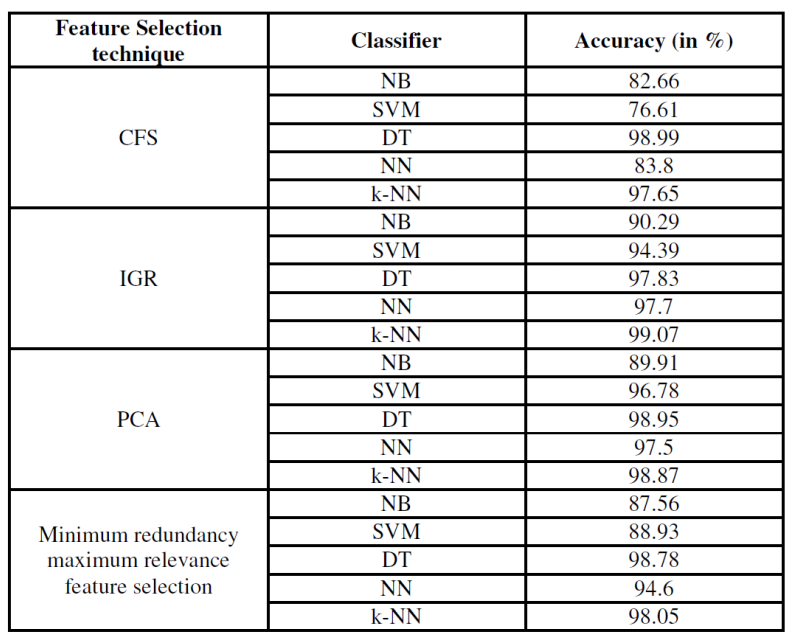
\includegraphics[width=\textwidth]{img/Comparison.png}
\end{figure}
\chapter{IDS Implementation}

Let's get serious now! An overview of IDS and how statistical techniques can be used with it has been proposed the next step is how to make all these things working together and what are the problems when you go from theory to practice!\newline\newline
In this example, it has been used the KDDCUP99 dataset, a well known set of network data collected by a military company\newline
The steps one must follow in order to build a good system, both in intrusion detection efficiency and computational efficiency are the followings:
\begin{itemize}
	\item[1)] \textbf{Data preprocess} - In this step the main issue is that most of the times data are numbers and strings mixed together. A numerical representation for all the strings in the dataset is mandatory for the next steps
	\item[2)] \textbf{Data standardization/normalization} - At this point, if we observe the dataset D, it can be seen that the range of numbers in D is not uniform. What must be done here is to run an algorithm that produces an output consisting of a new dataset D' where the values are standardized (or normalized, according to your needs)
	\item[3)] \textbf{Decision Tree method} Last step. The classification tool (the Decision Tree in this case) must be fed with the new dataset D' to build the data structure that will be then used to detect intrusions and malicious behaviours
\end{itemize}

A visual model for these steps is given in the next figure.

\begin{figure}[h!]
	\centering
	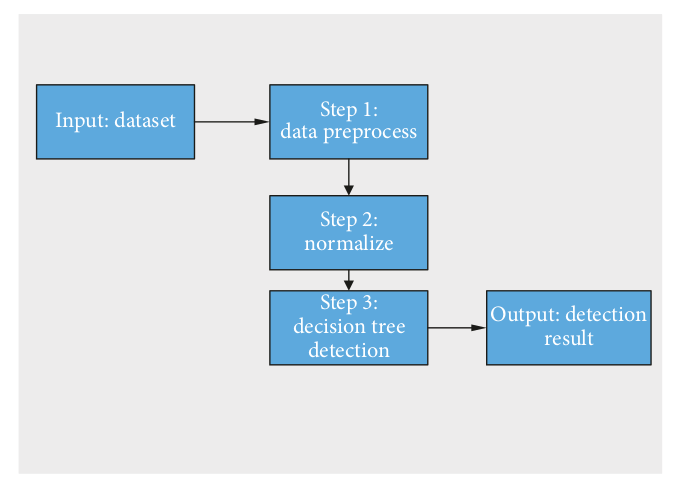
\includegraphics[width=\textwidth]{img/Steps.png}
\end{figure}

\begin{minipage}{\linewidth}
\vspace{0.5cm}
So, the first step is to preprocess data in order to work with them. This step is nothing but technical and requires really little skills

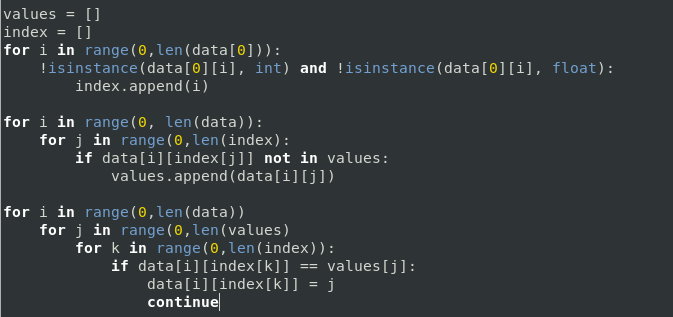
\includegraphics[width=\textwidth]{img/PreprocessCode.png}

\end{minipage}

\vspace{0.5cm}

At this point, there is the need to standardize the data in order to be able to do the Principal Component Analysis. This is a very important step because, if wrongly implemented, it can really blast down the accuracy of predictions.\newline
Standardizing data mean that the new dataset must have all the distributions associated to the features with mean = 0 and variance = 1.\newline\newline
Luckily, there is a python library that implements a lot of these features for us: the Pandas library.\newline\newline
The very important drawback here is that we can't standardize the train-set and the test-set separately (or the accuracy of prediction will be mined): the train-set must be standardized first and the same criteria must be used to standardize the test-set as well. In other words: the scaler must be "fit" using the train-set and then use the \emph{same} scaler to apply the transformation to both sets\newline\newline
\vspace{0.3cm}
\begin{minipage}{\linewidth}

	\centering
	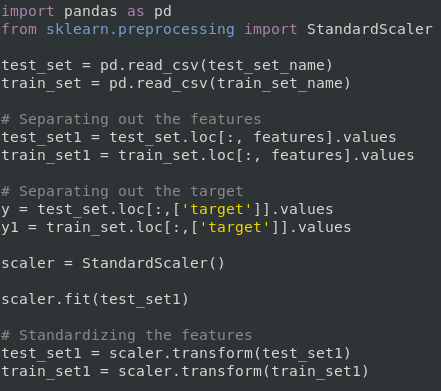
\includegraphics[width=\textwidth]{img/Normalization.png}
\end{minipage}

\vspace{0.5cm}

\begin{minipage}{\linewidth}
At this point, Principal Component Analysis algorithm can be run in order to exclude those features that have little significance for our purpose:\newline\newline

	\centering
	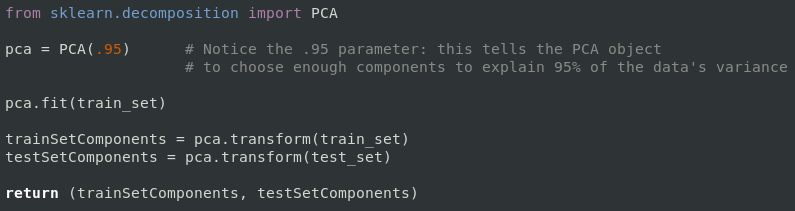
\includegraphics[width=\textwidth]{img/PCA.png}
	
	\vspace{0.5cm}

Now that data have been cleaned, standardized, and the features reduced those that are the most relevant, they can be used to feed the Decision Tree algorithm!\newline\newline
For the Tree construction the \emph{rpart} package has been used, due to its acceptance in statistical/machine learning environments. It is also quite efficient and let the user specify a lot of useful parameters for the tree construction.\newline In the next few lines, the algorithm used to build a Decision Tree is briefly described:

\begin{itemize}
	\item[1)] For each variable the whole dataset is split in 2 parts, using the Gini Index
		\begin{itemize}
			\item[$\rightarrow$] Since the variables are somehow continuous, splits will be done on boolean conditions: given a \emph{threshold t} features will be split according to the ones greater than \emph{t}, or lower than \emph{t}
		\end{itemize}
	\item[2)] The variable (or feature) that produced the highest score (the lowest Gini Index) will be the very first split of the Tree (the root node)
	\item[3)] The algorithm now proceeds recursively on each node, until there are no more variable to split
\end{itemize}

	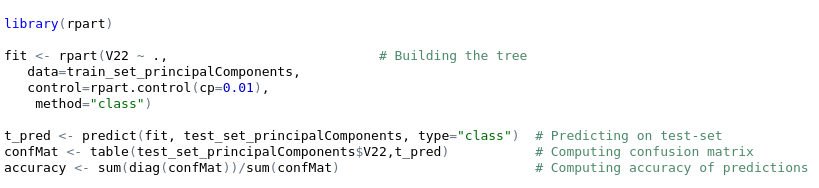
\includegraphics[width=\textwidth]{img/Rpart.png}
	
\end{minipage}

\vspace{0.5cm}

\begin{minipage}{\linewidth}

	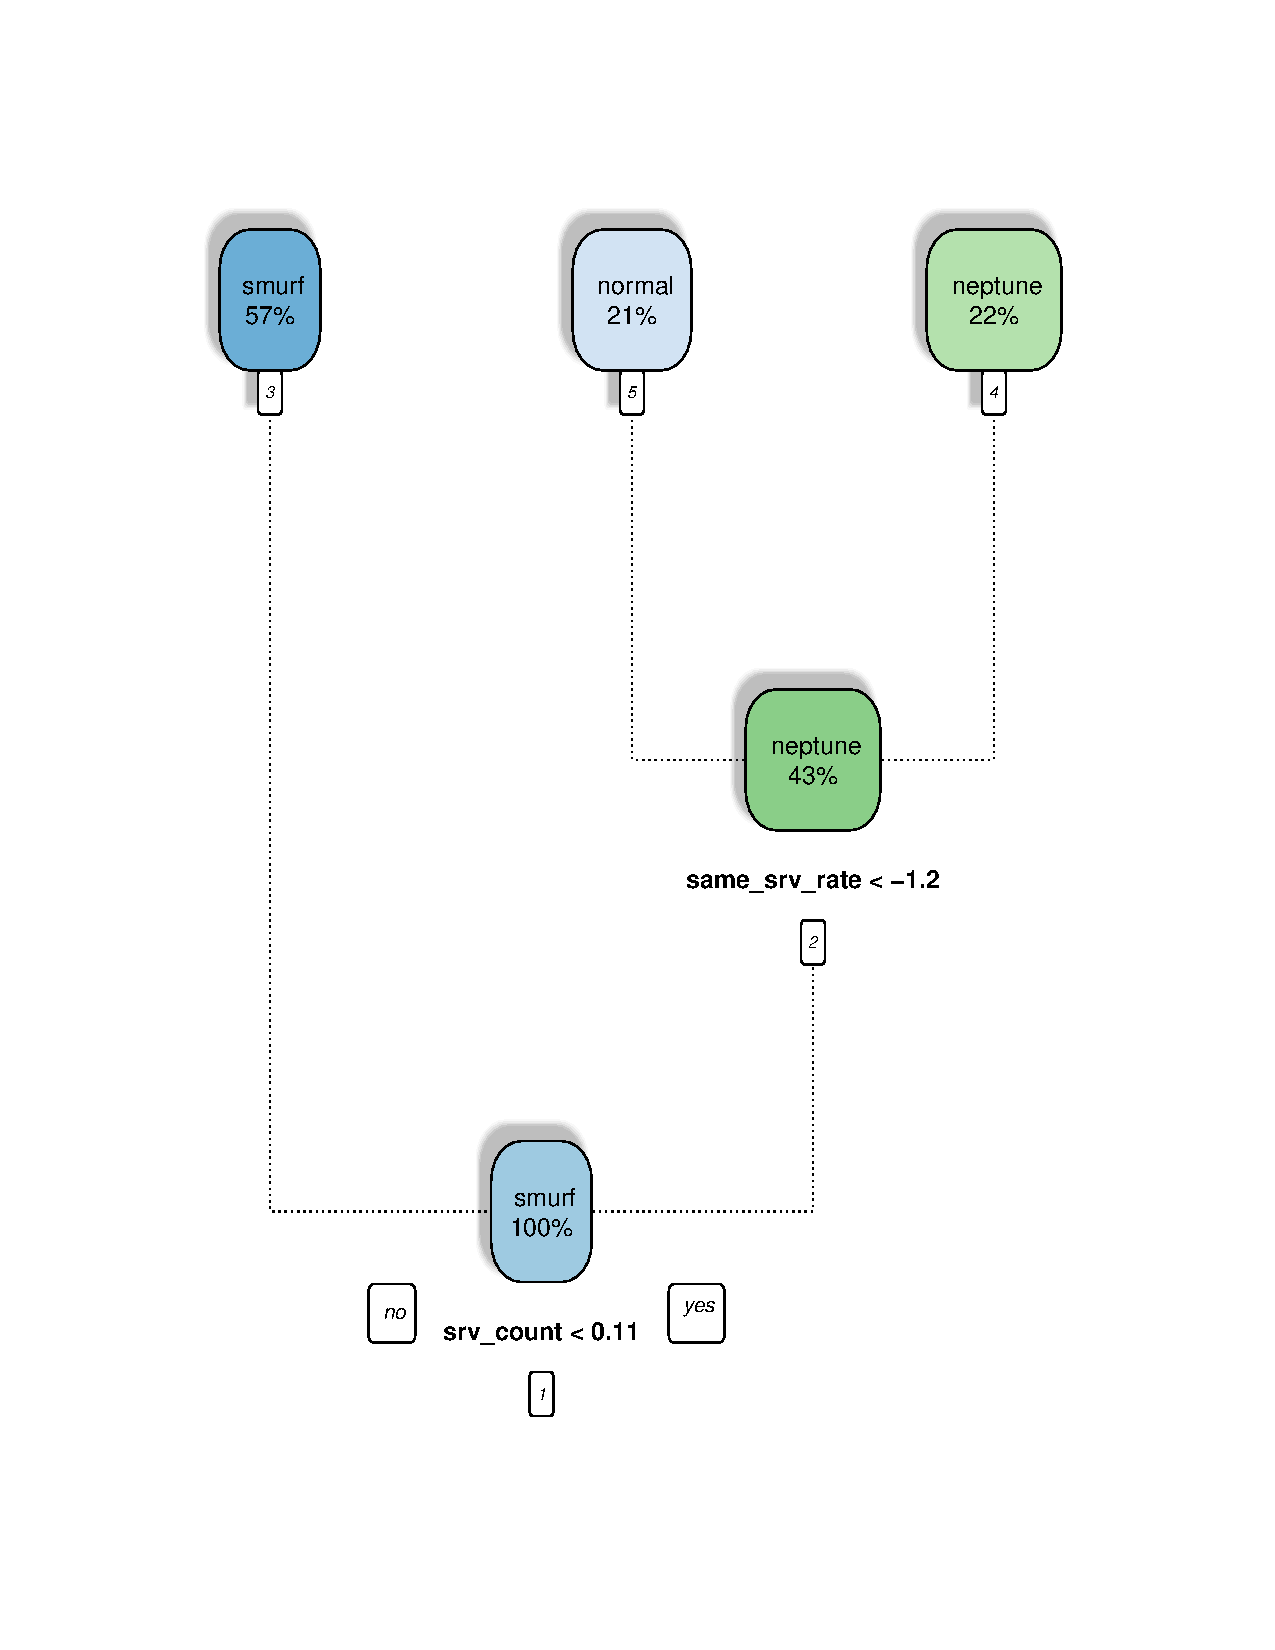
\includepdf{img/RplotStupido.pdf}
	Small and simple tree example to be read bottom-up
	
\end{minipage}
	
\chapter{Results \& Conclusions}

Now that that all the technical things are done we can run our algorithm to see its accuracy.\newline\newline
For empirical purposes, the algorithm have been run with different train-set and with different settings (e.g. complexity parameter), in order to see the differences between an analysis with and without principal components.\newline
Before showing the results here there are some technical data:\newline

The complexity parameter for the tree construction was set to 0.01, 0.0025 and 0.001 and train-sets were:\newline

\begin{itemize}
	\item[1)] Standardized set, using all the features
	\item[2)] Standardized set, using only the features \emph{selected} by PCA (that is, indeed, a non-standard use of this technique)
	\item[3)] The new set of features \emph{produced} by PCA
\end{itemize}

Regarding test and train set:

\begin{itemize}
	\item The train-set is the 10\% of the Kddcup dataset (which is much much lower than the "standard" dimension, which usually is around 70/80\%)
	\item The test-set is the \emph{whole} Kddcup dataset, consisting of 42 features with almost 5 millions values
	\item When the PCA train-set was used, the test-set was transformed accordingly to the transformations done on the test-set (remember we had to "fit" the scaler with pandas?)
\end{itemize}

Results and some of the plots are shown in the next figures:


\begin{center}
	{\setlength{\extrarowheight}{20pt}
	\begin{tabular}{| c | c | c | c |}
	\hline
		Complexity parameter & 0.01 & 0.0025 & 0.001 \\ \hline
		StandardizedKddcup & 0.9870385 & 0.9832191 & 0.9843356 \\ \hline
		KddcupPrincipalFeatures & 0.9849946 & 0.9948412 & 0.9963878 \\ \hline
		PCA eigenvectors & 0.9901552 & 0.9951242 & 0.9956888 \\ 
		\hline
	\end{tabular}}
\end{center}

\vspace{0.3cm}

If we observe data we can see how Principal Component Analysis raises the accuracy of our prediction. Moreover, the trees built using the selected components are much more balanced when we increase the complexity parameter (i.e. we build bigger trees), while using all the features we get an unbalanced tree.\newline\newline
Another thing to point out is that, with a c.p. of 0.001 we get more accuracy if we don't use the new features produced by PCA (but this could be a matter of the dimension of the train-set)\newline\newline
To conclude, it has been observed that PCA is indeed a useful technique to improve the overall accuracy of predictions in Decision Trees (and it also fasten execution time since we have less features!). For future works, considerations may be done regarding Random Forest (i.e. Distributed IDS) and how to combine it with PCA.\newline\newline
\clearpage
In the following pages there are some plots of the various Decision Tree in order to appreciate the differences between the ones that used PCA and the ones that didn't.
\vspace{2cm}

\begin{itemize}


	\item[Figure 1 - ]This is the tree built with the whole features-set, with a c.p. = 0.0025. As can be seen it is very unbalanced. The more complex is the model, the more unbalanced is the tree


	\item[Figure 2 - ]This is the tree built using the new features produced by PCA. Compared to the previous one, it is much more balanced (and accurate!)


	\item[Figure 3 - ]Just for some fun, this is the (very big) tree, built using PCA's features with a c.p. = 0.001


	\item[Figure 4 - ]And here it is the DT built with the whole feature-set and a c.p. = 0.001. As can be seen, things exhacerbate when we try to build complex models, while using PCA we get better data structures	
\end{itemize}

\clearpage
\afterpage{
\begin{minipage}{\linewidth}
Figure 1
	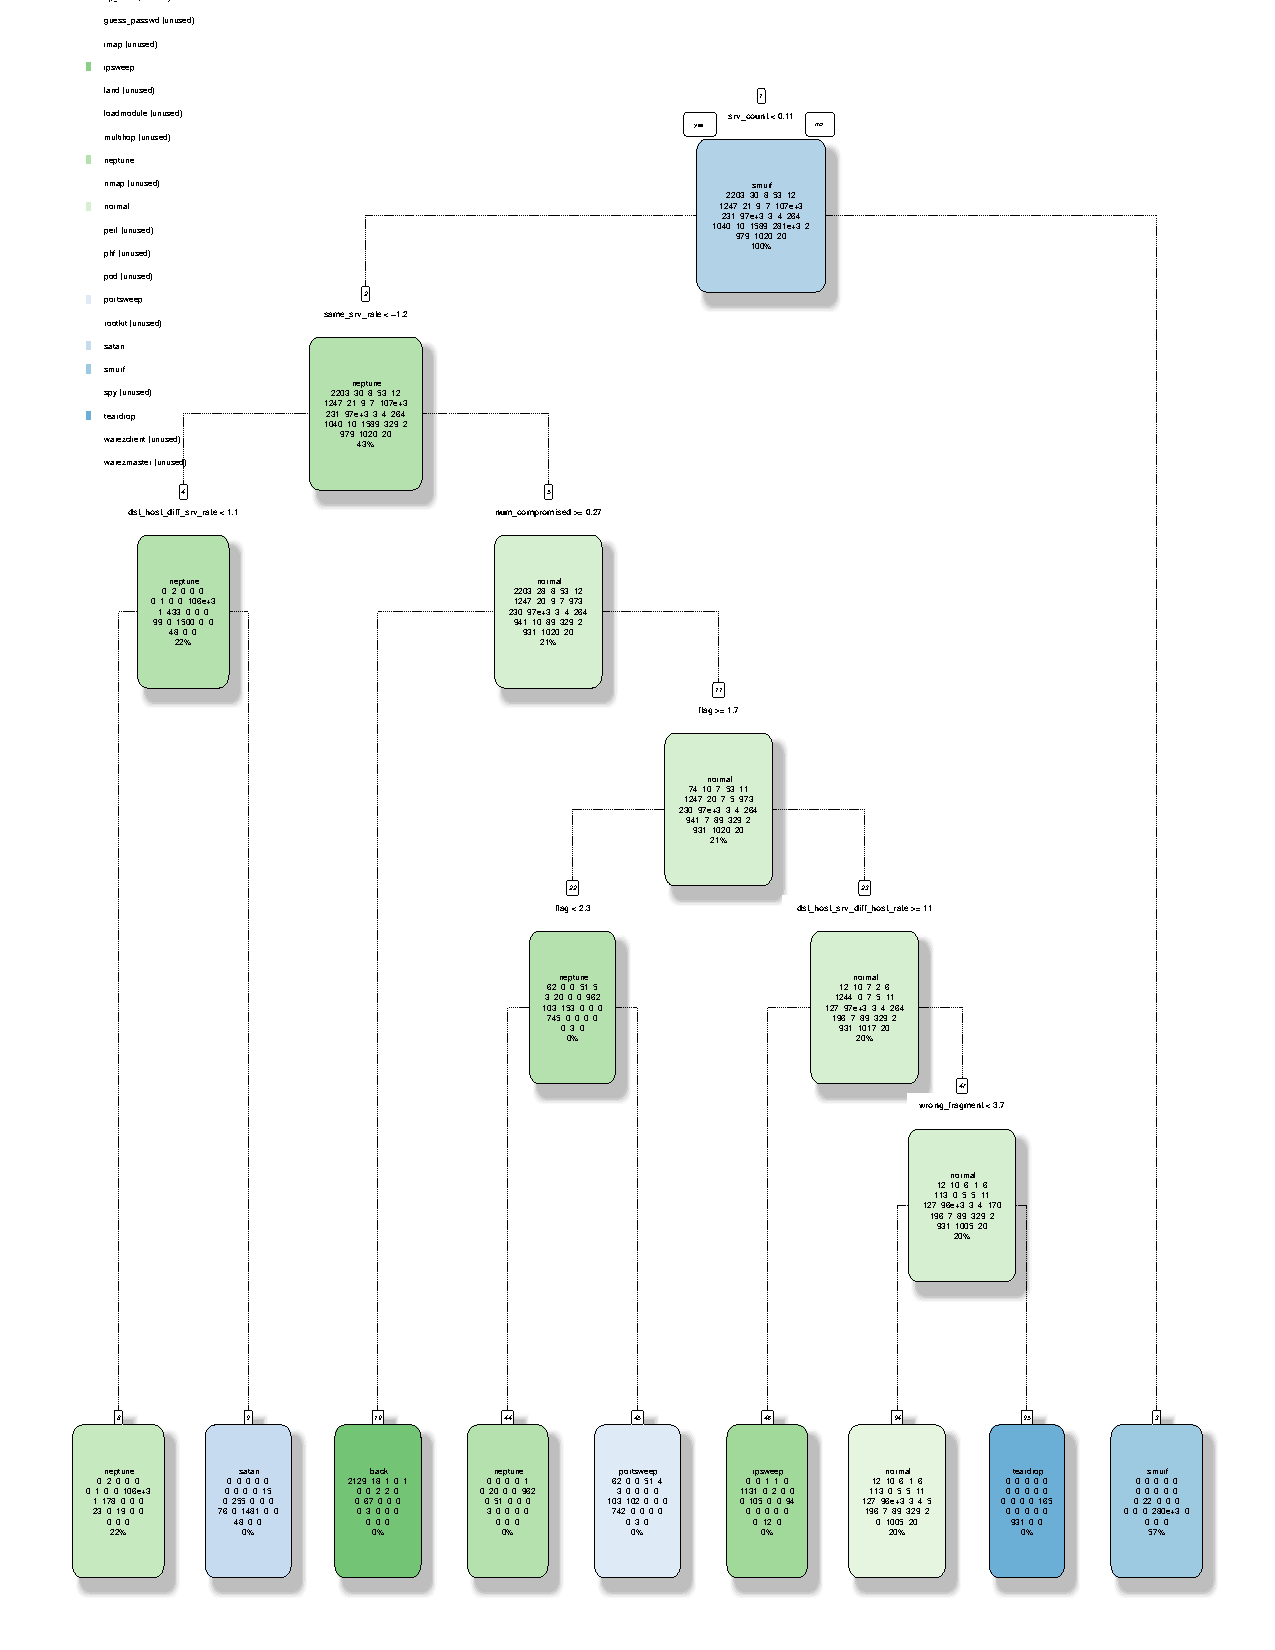
\includepdf{img/noncomponents0025.pdf}
\end{minipage}
}
\clearpage
\afterpage{
\begin{minipage}{\linewidth}
Figure 2
	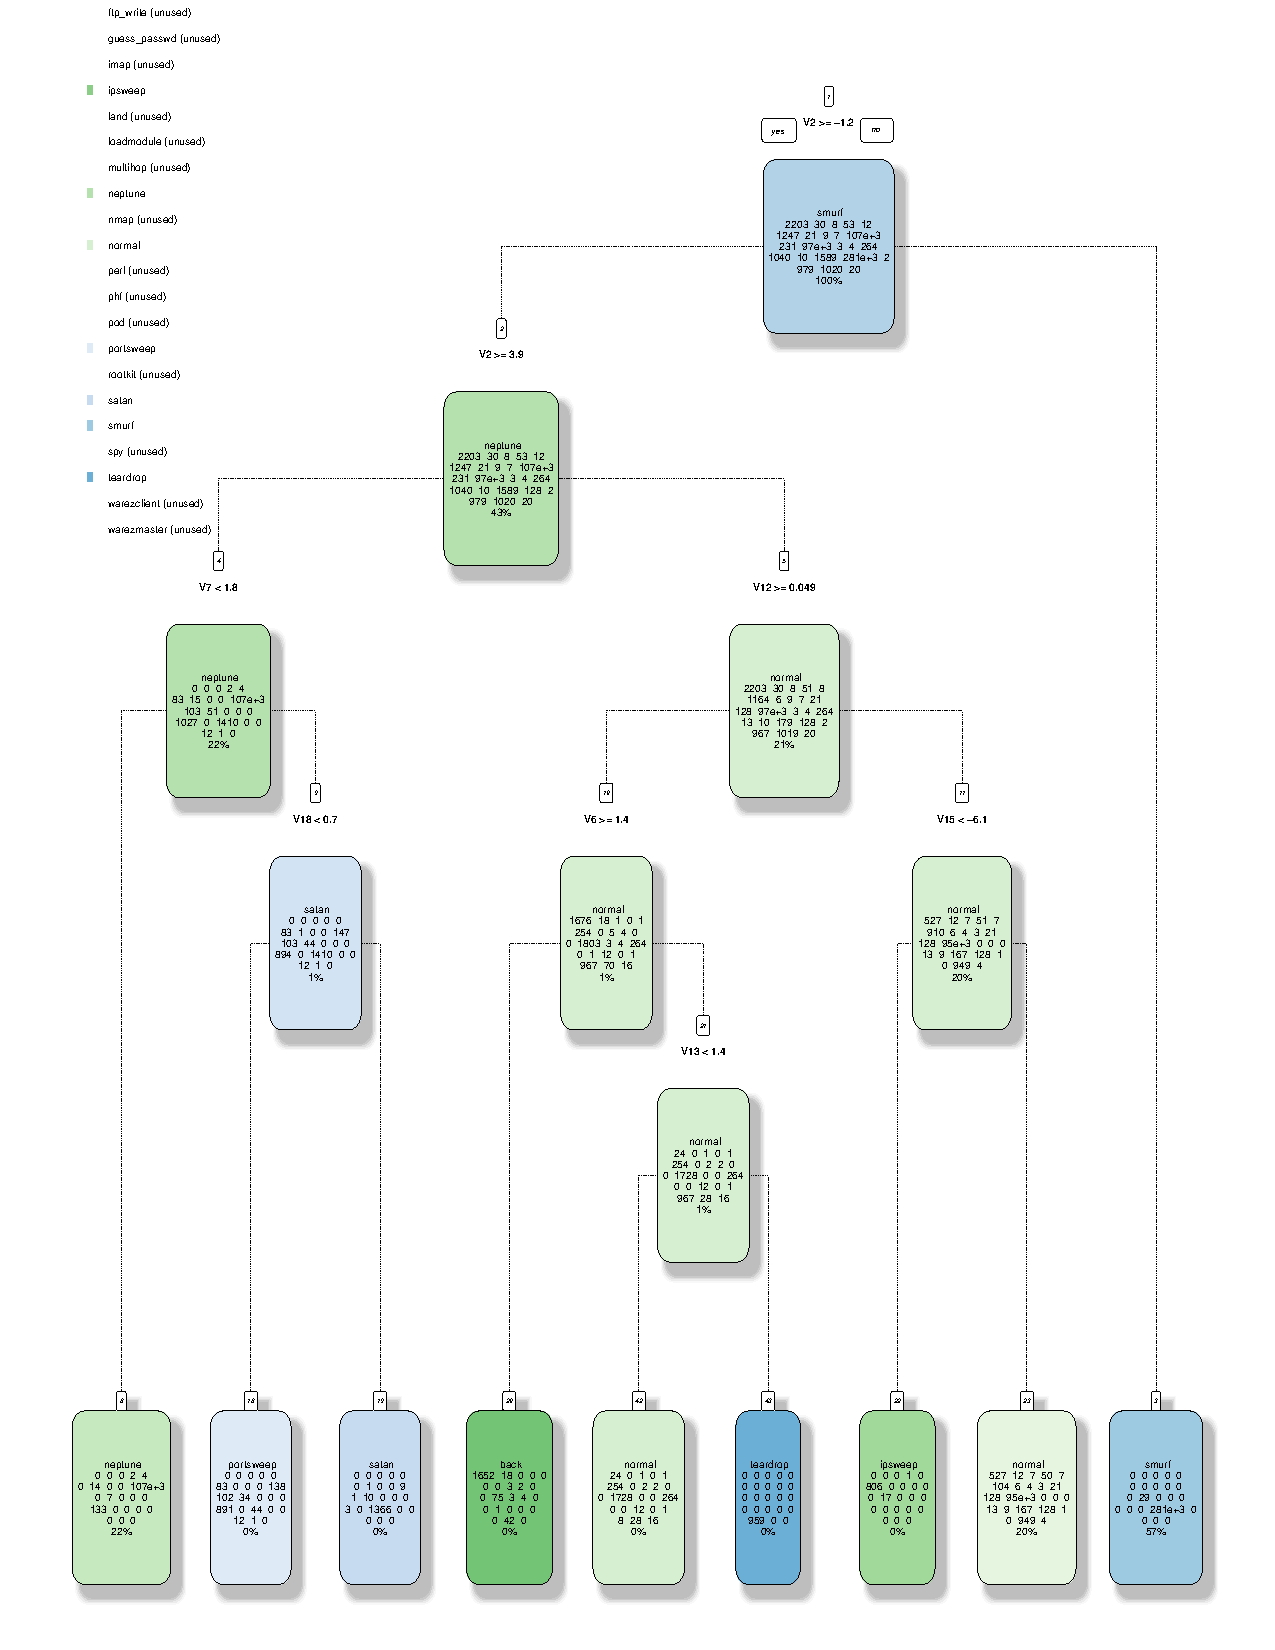
\includepdf{img/components0025.pdf}
\end{minipage}
}
\clearpage
\afterpage{
\begin{minipage}{\linewidth}
Figure 3
	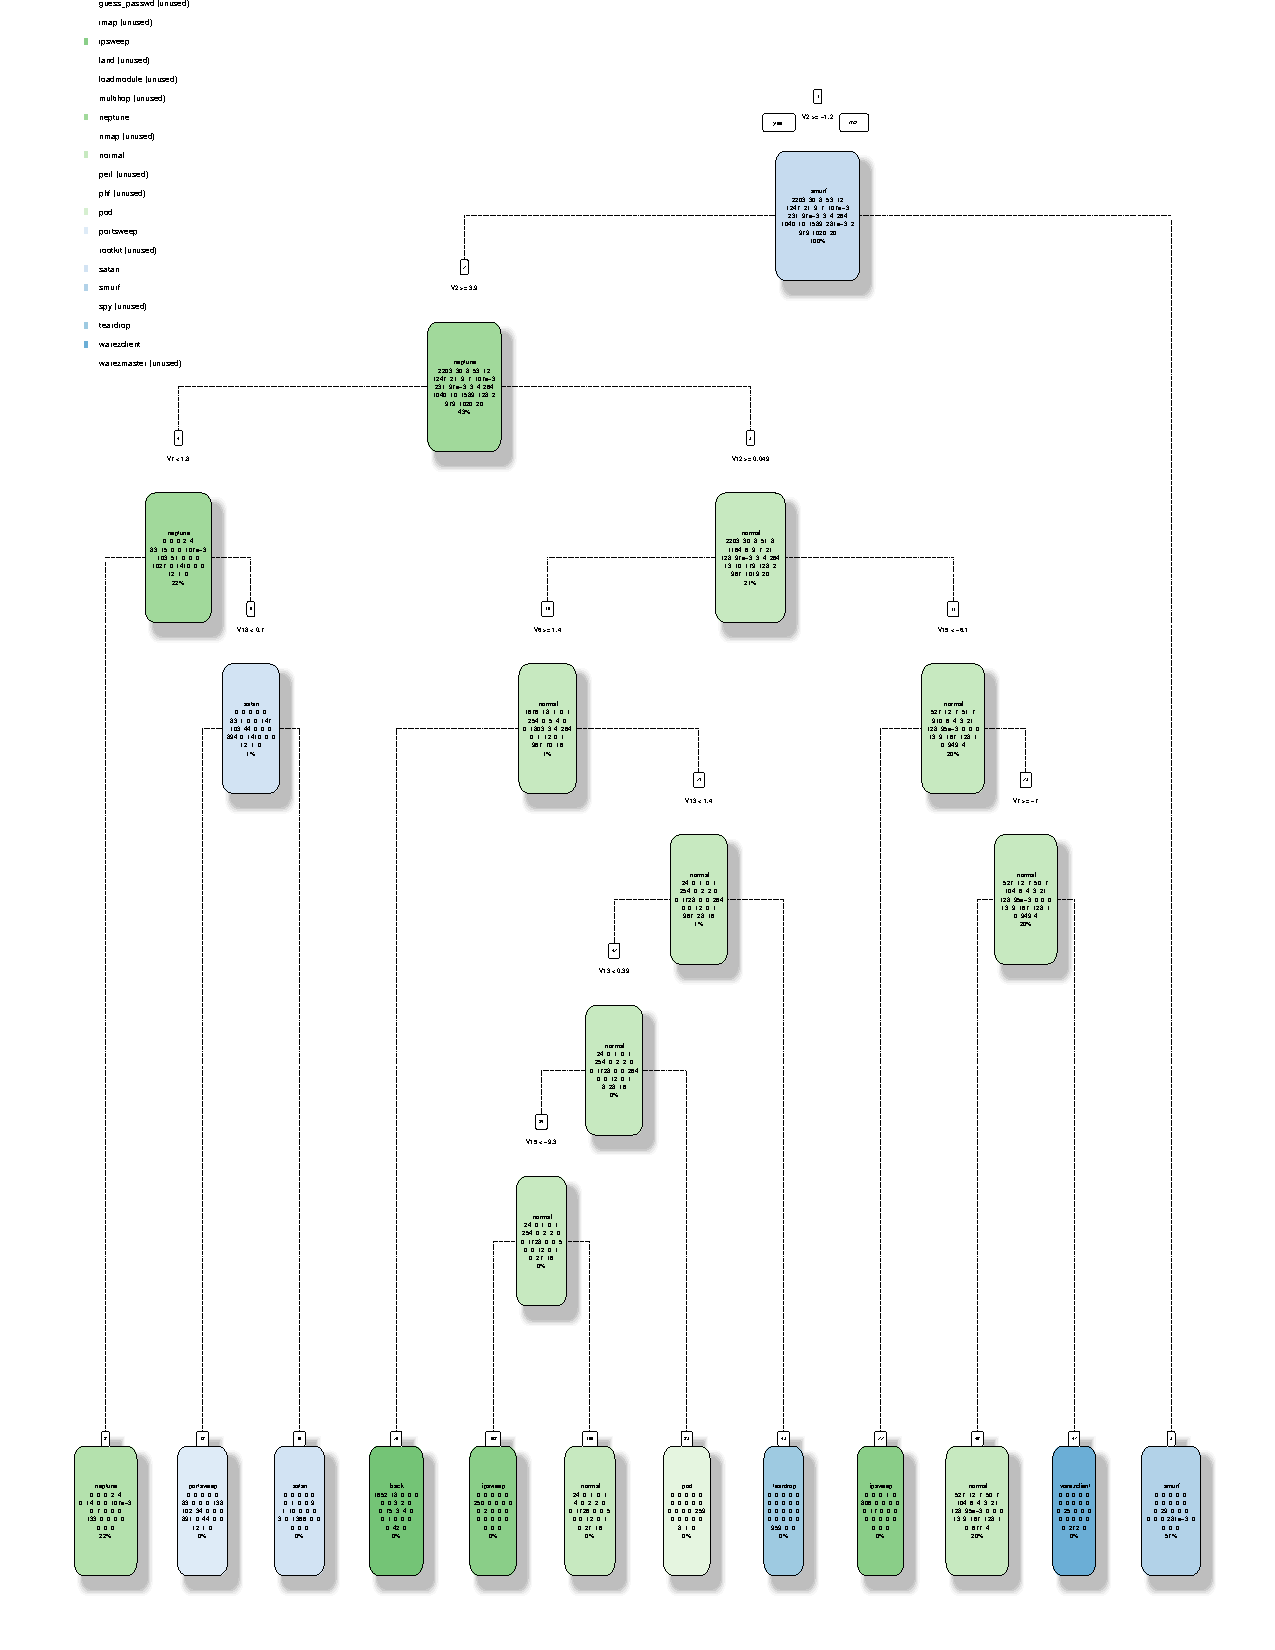
\includepdf{img/components001.pdf}
\end{minipage}
}
\clearpage
\afterpage{
\begin{minipage}{\linewidth}
Figure 4
	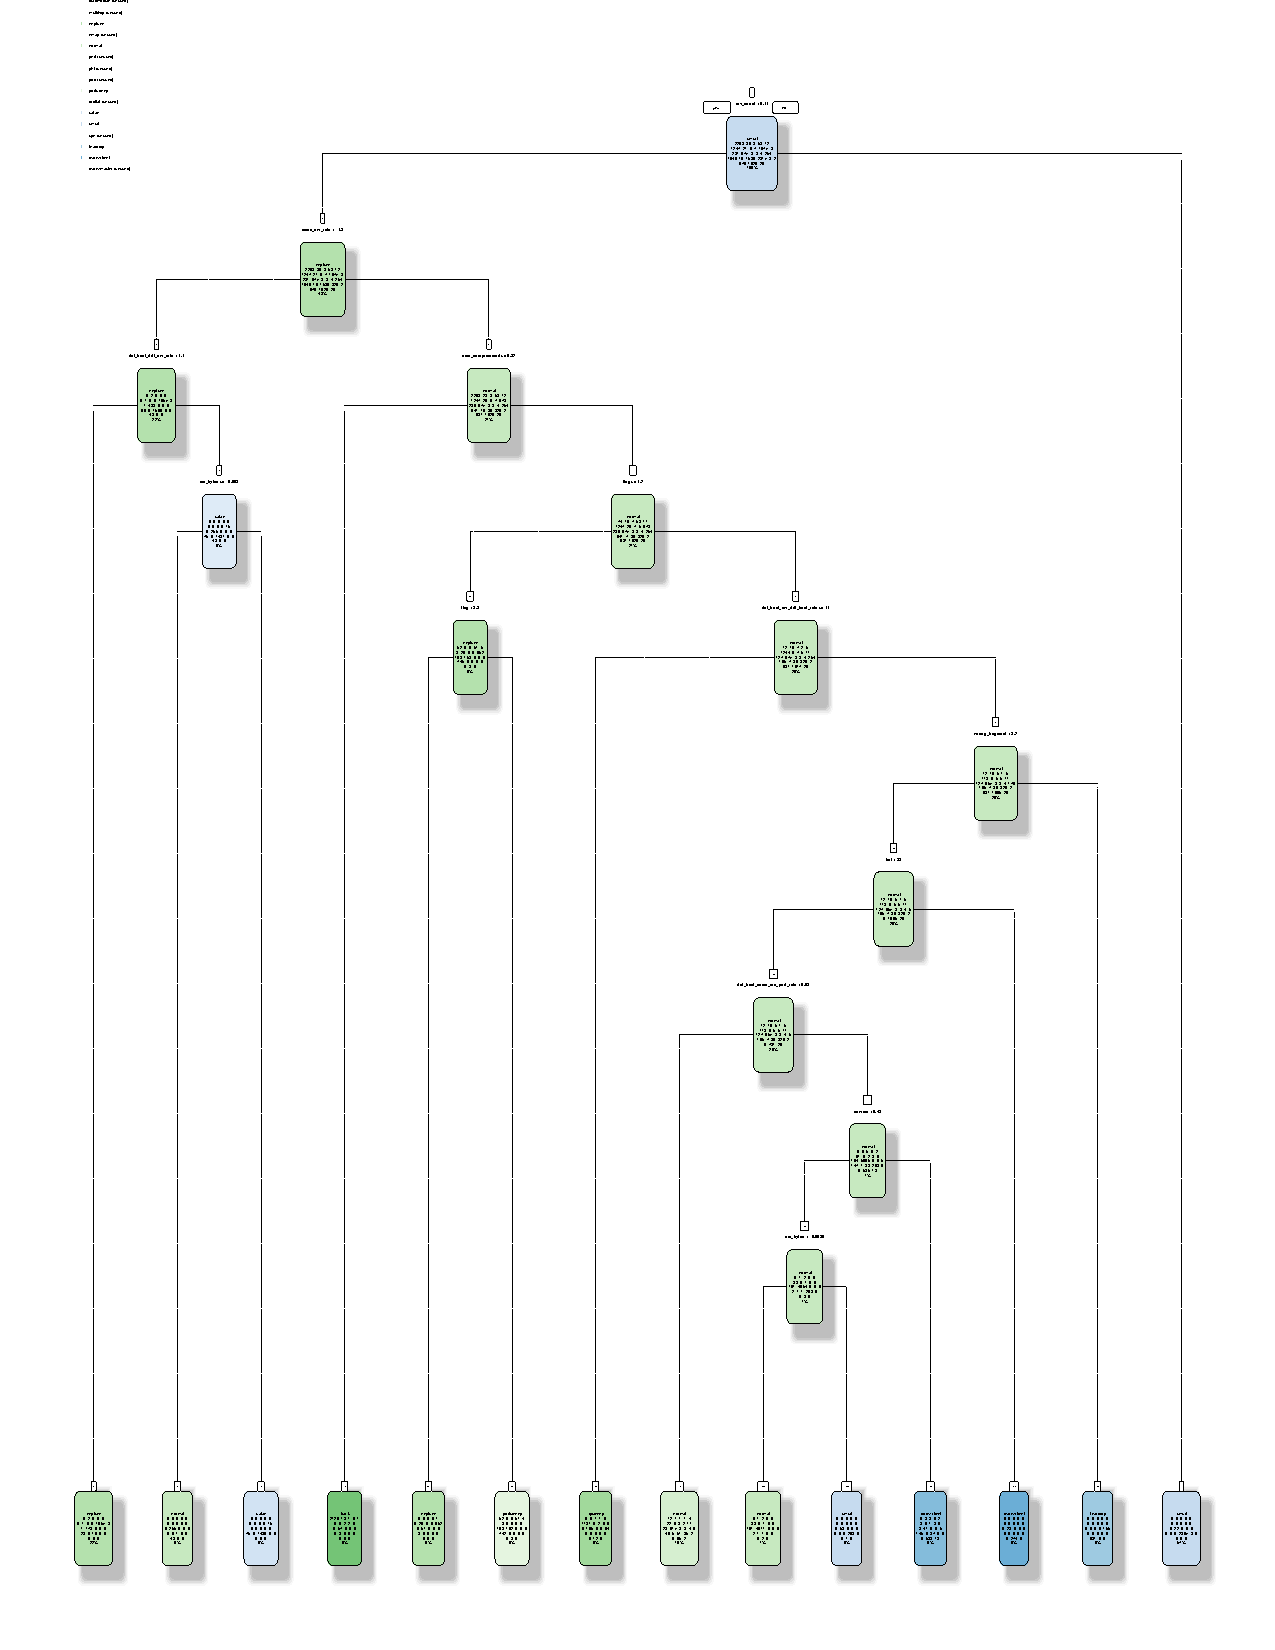
\includepdf{img/noncomponents001.pdf}
\end{minipage}
}
\begin{thebibliography}{99}

\bibitem{bibitem1}{Saroj Kr. Biswas - \emph{Intrusion Detection Using Machine Learning: A Comparison Study}}

\bibitem{bibitem2}{Kai Peng, Victor C. M. Leung, Lixin Zheng, Shangguang Wang, Chao Huang, Tao Lin - \emph{Intrusion Detection System Based on Decision Tree over Big Data in Fog Environment}}

\end{thebibliography}

%--------------------------------------------------------------
\end{document}
%--------------------------------------------------------------
